\chapter{Calculus}

\section{Difference Quotient ( $\displaystyle\frac{\delta y}{\delta x}$ )}\label{Difference Quotient}

\begin{table}[H]
    \begin{minipage}{0.39\linewidth}
        \begin{figure}[H]
            \centering
            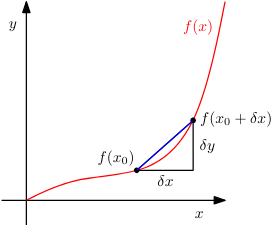
\includegraphics[height=4cm]{Pictures/maths/Difference Quotient.png}
            \caption{Difference Quotient}
        \end{figure}
    \end{minipage}
    \hfill
    \begin{minipage}{0.59\linewidth}
        \begin{enumerate}
            \item The difference quotient \( \displaystyle\dfrac{\delta y}{\delta x} = \displaystyle\dfrac{f(x + \delta x) - f(x)}{\delta x} \) computes the slope of the secant line through two points on the graph of $y = f(x)$. 
            
            \item The difference quotient can also be considered the average slope of $f$ between $x$ and $x + \delta x$ if we assume $f$ to be a linear function. 
            
            \item In the limit for $\delta x \rightarrow 0$, we obtain the tangent of $f$ at $x$, if $f$ is differentiable.

        \end{enumerate}
    \end{minipage}
\end{table}



\section{Derivative ( $\displaystyle\frac{dy}{dx}$ / $y'$)}\label{Derivative}

For $h > 0$ the derivative of $y = f(x)$ at $x$ is defined as the limit \( \displaystyle\dfrac{\delta y}{\delta x} = \lim_{h\rightarrow 0}\displaystyle\dfrac{f(x + h) - f(x)}{h} \) and the secant becomes a tangent.

\subsection{Sum rule}
\[
    (f(x) + g(x))' = f'(x) + g'(x)
\]

\subsection{Product rule}
\[
    (f(x)g(x))' = f'(x)g(x) + f(x)g'(x)
\]

\subsection{Chain rule}
\[
    g(f(x))' = (g \circ f)'(x) = g'(f(x))f'(x)
\]

\subsection{Quotient rule}
\[
    \dParenBrac{ \displaystyle\dfrac{f(x)}{g(x)} }' = \displaystyle\dfrac{[f'(x)g(x) - f(x)g'(x)]}{(g(x))^2}
\]


\section{directional derivative \cite{dnn-deep-learning-ian}} \label{directional derivative}

\begin{enumerate}
    \item The directional derivative in direction $u$ (a unit vector) is the slope of the function $f$ in direction $u$. 
    
    \item In other words, the directional derivative is the derivative of the function $f(x + \alpha u)$ with respect to $\alpha$, evaluated at $\alpha = 0$. 
    
    \item Using the chain rule, we can see that $\dfrac{\partial}{\partial\alpha} (x+\alpha u)$ evaluates to $u^\top\nabla_xf(x)$ when $\alpha = 0$.

    \item To minimize $f$, we would like to find the direction in which $f$ decreases the fastest. We can do this using the directional derivative:
    \[
        \min_{u,u^\top u = 1} u^\top \nabla_x f(x)
        = \min_{u,u^\top u = 1} \dnorm{u}_2 \dnorm{\nabla_x f(x)}_2 \cos{(\theta)}
    \]
    where $\theta$ is the angle between $u$ and the gradient.
\end{enumerate}




\section{Power Series}\label{Power Series}
\[
    f(x) = \sum_{k=0}^{\infty} a_k (x-c)^k
\]
where $a_k$ are coefficients and $c$ is a constant

\section{Taylor Polynomial ( $T_n(x)$ )}\label{Taylor Polynomial}
The Taylor polynomial of degree $n$ of $f : \mathbb{R} \rightarrow \mathbb{R}$ at $x_0$ is defined as: 
\[
    T_n(x) = \sum_{k=0}^{n}\displaystyle\dfrac{f^{(k)}(x_0)}{k!}(x-x_0)^k
\]
where, $f^{(k)}(x_0)$ is the $k$th derivative of $f$ at $x_0$ and $\displaystyle\dfrac{f^{(k)}(x_0)}{k!}$ are the coefficients of the polynomial.


\section{Multivariate Taylor Polynomial}\label{Multivariate Taylor Polynomial}
The Taylor polynomial of degree $n$ of $f$ at $x0$ contains the first $n + 1$ components of the series and is defined as:
\[
    f(x) = \sum_{k=0}^{n} \displaystyle\dfrac{D_x^k f(x_0)}{k!}\delta^k
\]

where, $D_x^kf(x_0)$ is the $k$-th (total) derivative of $f$ with respect to $x$, evaluated at $x_0$.

$k$th-order tensor \( \delta^k \in \mathbb{R}^{\overset{k \text{ times}}{\overbrace{D \times D \times \cdots \times D}}} \) is obtained as a $k$-fold outer product, denoted by $\bigotimes$, of the vector $\delta \in \mathbb{R}^D$

\begin{table}[H]
    \centering
    \begin{tabular}{l l}
        \( \delta^2 := \delta\bigotimes\delta = \delta\delta^\top \) & \( \delta^2[i, j] = \delta [i]\delta [j] \) \\
        \( \delta^3 := \delta\bigotimes\delta\bigotimes\delta \) & \( \delta^3[i, j, k] = \delta [i]\delta [j]\delta [k] \) \\
    \end{tabular}
\end{table}

$D_x^kf(x_0)\delta k$ contains $k$-th order polynomial:
\begin{table}[H]
    \begin{tabular}{l l}
        $k = 0$ & $D_x^0f(x_0)\delta^0 = f(x_0) \in \mathbb{R}$ \\
         
        $k = 1$ & \( D_x^1f(x_0)\delta^1 = \underbrace{\nabla_xf(x_0)}_{1\times D} \underbrace{\delta}_{D \times 1} = \dsum_{i=1}^{D} \nabla_xf(x_0)[i]\delta [i] \in \mathbb{R} \) \\

        $k = 2$ & \( D_x^2f(x_0)\delta^2 = \operatorname{tr}(\underbrace{H(x_0)}_{D\times D} \underbrace{\delta}_{D \times 1} \underbrace{\delta^\top}_{1 \times D}) = \delta^\top H(x_0)\delta = \dsum_{i=1}^{D}\dsum_{j=1}^{D} H[i,j]\delta [i]\delta [j] \in \mathbb{R} \) \\

        $k = 3$ & \( D_x^3f(x_0)\delta^3 = \dsum_{i=1}^{D} \dsum_{j=1}^{D} \dsum_{k=1}^{D} D_x^3f(x_0)[i,j,k]\delta [i] \delta [j] \delta [k] \in \mathbb{R} \) \\
         
    \end{tabular}
\end{table}

$H(x_0)$ is the \textbf{Hessian} of $f$ evaluated at $x_0$.


\section{Taylor Series ( $T_\infty(x)$ )}\label{Taylor Series}
For a smooth function $f \in C^\infty$, $f : \mathbb{R} \rightarrow \mathbb{R}$, the taylor series of $f$ at $x_0$ is defined as:

\[
    T_\infty(x) = \sum_{k=0}^{\infty}\displaystyle\dfrac{f^{(k)}(x_0)}{k!}(x-x_0)^k
\]

SEE: \fullref{Taylor Polynomial}
\begin{enumerate}
    \item $f^{(k)}(x_0)$ is the $k$th derivative of $f$ at $x_0$

    \item For $x_0 = 0$, we obtain the \textbf{Maclaurin series}\indexlabel{Maclaurin series} as a special instance of the Taylor series. 
    
    \item If $f(x) = T_\infty(x)$, then $f$ is called \textbf{analytic}\indexlabel{analytic}.
    
    \item $f \in C^\infty$ means that $f$ is continuously differentiable infinitely many times.

    \item a Taylor polynomial of degree $n$ is an approximation of a function, which does not need to be a polynomial

    \item The Taylor polynomial is similar to $f$ in a neighborhood around $x_0$. However, a Taylor polynomial of degree $n$ is an exact representation of a polynomial $f$ of degree $k \leq n$ since all derivatives $f(i)$, $i > k$ vanish.

    \item it is a special case of \textbf{power series}(SEE: \fullref{Power Series}).

\end{enumerate}


\section{Multivariate Taylor Series}\label{Multivariate Taylor Series}

SEE: \fullref{Multivariate Taylor Polynomial}\\
We consider a function $f : \mathbb{R}^D \rightarrow \mathbb{R}$, $x \rightarrow f(x)$, $x \in \mathbb{R}^D$, that is smooth at $x_0$. When we define the difference vector $\delta := x - x_0$, the multivariate Taylor series of $f$ at $x_0$ is defined as
\[
    f(x) = \sum_{k=0}^{\infty} \displaystyle\dfrac{D_x^k f(x_0)}{k!}\delta^k
\]

where, $D_x^kf(x_0)$ is the $k$-th (total) derivative of $f$ with respect to $x$, evaluated at $x_0$.






























































































